%!TEX encoding = UTF-8 Unicode
% coding: utf-8

%!TEX encoding = UTF-8 Unicode
% coding: utf-8
% Header per le presentazioni in LaTeX+beamer
% @author Eric Miotto
% @date 15/12/2006

\documentclass{beamer}

%Configurazione beamer
\mode<presentation>
{
 %Tema grafico
  \usetheme{Frankfurt}
  
  %Colori da usare per il tema
  \usecolortheme{seahorse} 
  \usecolortheme{rose} 

  \setbeamercovered{transparent}
}

%Importazione package
\usepackage[italian]{babel} %Lingua e sillabazione in italiano
\usepackage[utf8]{inputenc} %Codifica UTF8
\usepackage{textpos} %Posizionamento testo e immagini ovunque sulla pagina

% Griglia di posizionamento delle immagini
% Il primo parametro sono il numero di colonne in cui viene diviso il foglio,
% il secondo sono il numero di righe in cui viene diviso il foglio
%\TPGrid{3}{1}

\title{Considerazioni finali (si spera..) \\ su C04}

\author{Egoless Group}

\date[RA 28/03/2007] % (optional, should be abbreviation of conference name)
{Revisione di Accettazione \\ 28 marzo 2007}

\subject{Presentazione del prodotto per il capitolato C04}

\logo{
\includegraphics[width=1cm]{img/logo.jpg}}

% Delete this, if you do not want the table of contents to pop up at
% the beginning of each subsection:

%Ci pensa lui a creare l'indice

%\AtBeginSubsection[]
%{
%  \begin{frame}<beamer>
%    \frametitle{Outline}
%    \tableofcontents[currentsection,currentsubsection]
%  \end{frame}
%}

\AtBeginSection[]
{
  \begin{frame}<beamer>
    \frametitle{Outline}
    \tableofcontents[currentsection]
  \end{frame}
}

\begin{document}

\begin{frame}
  \titlepage
\end{frame}

\begin{frame}
  \frametitle{Outline}
  \tableofcontents
  % You might wish to add the option [pausesections]
\end{frame}


% Structuring a talk is a difficult task and the following structure
% may not be suitable. Here are some rules that apply for this
% solution: 

% - Exactly two or three sections (other than the summary).
% - At *most* three subsections per section.
% - Talk about 30s to 2min per frame. So there should be between about
%   15 and 30 frames, all told.

% - A conference audience is likely to know very little of what you
%   are going to talk about. So *simplify*!
% - In a 20min talk, getting the main ideas across is hard
%   enough. Leave out details, even if it means being less precise than
%   you think necessary.
% - If you omit details that are vital to the proof/implementation,
%   just say so once. Everybody will be happy with that.

\section{Consuntivi}

\subsection*{Consuntivi per persona}

\begin{frame}
\frametitle{Consuntivi per persona}

\begin{figure}
  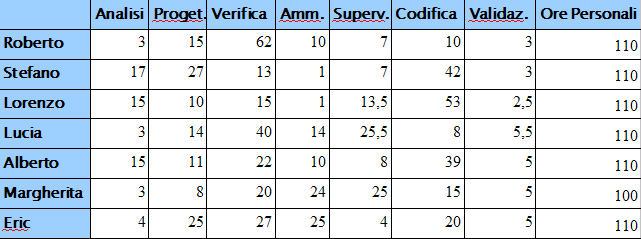
\includegraphics[width=10cm]{img/OrePersona.png}
\end{figure}

\end{frame}


\begin{frame}
\frametitle{Ore previste/Erogate}

\begin{figure}
  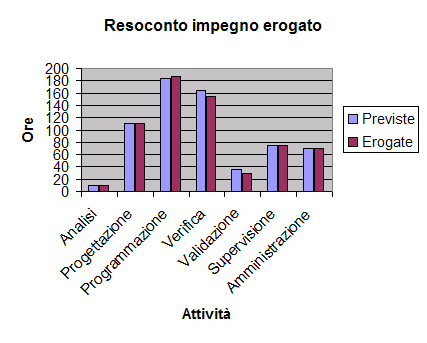
\includegraphics[width=10cm]{img/Impegno_Erogato.png}
\end{figure}

\end{frame}


\begin{frame}
\frametitle{Consuntivo finale di progetto}

\begin{figure}
  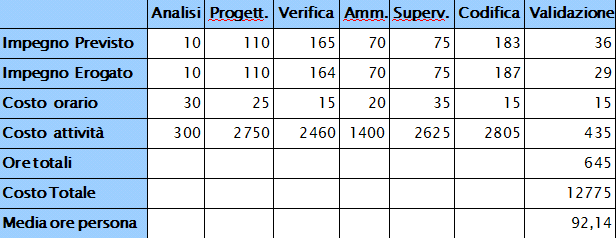
\includegraphics[width=10cm]{img/Consuntivo.png}
\end{figure}

\end{frame}


\section{In cosa abbiamo peccato}
\subsection*{In cosa abbiamo peccato}

\begin{frame}

\frametitle{In cosa abbiamo peccato}

\begin{quote}
``La comunicazione è fondamentale e dovrebbe occupare il 90\% del tempo del responsabile``
\end{quote}

\begin{flushright}
Ahmet Burdu, Capgemini
\end{flushright}

\begin{itemize}
\item pianificazione e scadenze con l'altro gruppo
\item i video del manuale utente, pronti, non sono stati allegati
\end{itemize}
\end{frame}


\subsection*{Cosa non avevamo previsto}
\begin{frame}
\frametitle{Cosa non avevamo previsto}

\begin{quote}
``I don't think anybody tests enough of anything``
\end{quote}

\begin{flushright}
James Gosling
\end{flushright}

\begin{itemize}
\item studio delle tecnologie più oneroso del previsto
\item rotazione dei ruoli dispendiosa
\item ..Murphy: l'ottavo componente..
\end{itemize}

\end{frame}

\section{Cosa non abbiamo sbagliato}
\subsection*{Cosa non abbiamo sbagliato}
\begin{frame}
\frametitle{Cosa \emph{non} abbiamo sbagliato}

\begin{itemize}
	\item capacità dell'architettura a web service ad integrarsi con cose già esistenti
	\item focalizzazione e risoluzione di problemi di uso comune  ``gestione studenti``, ``gestione professori``, quindi..
	\item ..buona base di partenza per i nostri eventuali successori
	\item semplicità di utilizzo
\end{itemize}
\end{frame}

\section{Espansioni future}
\subsection*{Espansioni future}
\begin{frame}

\frametitle{Espansioni future (da incontro con Zambello)}
\begin{itemize}
	\item rendere sicure le comunicazioni tra web service
	\item prevedere l'autenticazione degli utenti
	\item gestione monitoraggio e questionari
	\item piano di manutenzione
\end{itemize}
\end{frame}


\end{document}